\section{Versions}
\begin{itemize}
\item \begin{bf}Premi�re version\end{bf} : acc�der au menu
        \begin{itemize}
	\item afficher le fond anim� (2 couches)
	\item configurer le son (effets et musique)\\
        \end{itemize}

Voici un croquis du menu tel qu'il devra appara�tre � l'issue de la publication de la premi�re version :\\
\\
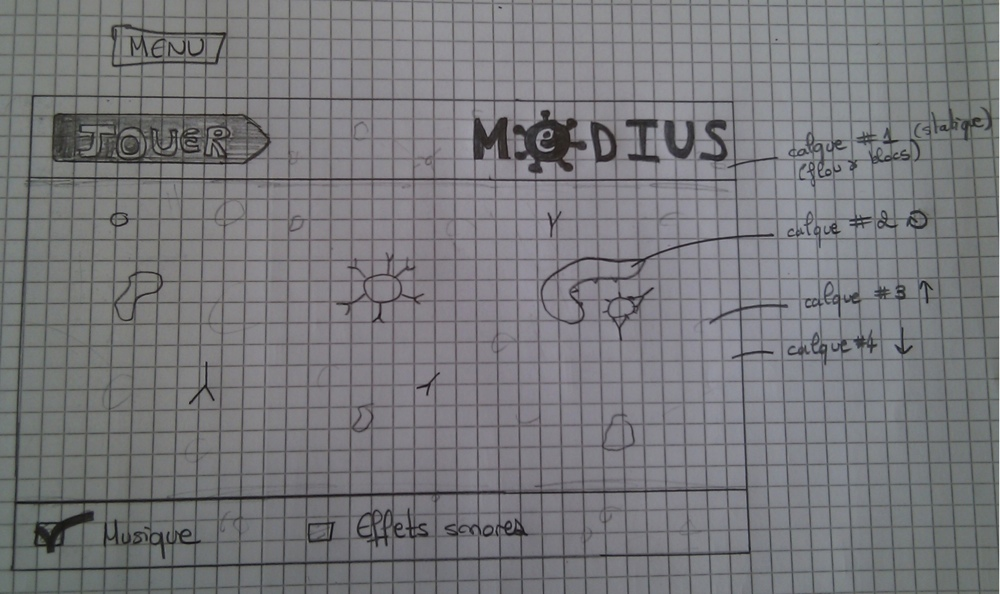
\includegraphics[scale=0.4]{Images/mockup_menu.jpg}
\\
\item \begin{bf}Deuxi�me version\end{bf} : acc�der aux niveaux
        \begin{itemize}
	\item afficher les niveaux
	\item lancer un niveau
	\item obtenir des d�tails sur un niveau (document d'aide)\\
        \end{itemize}
\item \begin{bf}Troisi�me version\end{bf} : acc�der aux combats \#1
	\begin{itemize}
	\item combattre une bact�rie
	\item afficher les organismes ennemis
	\item g�rer les tirs
	\item g�rer les cellules amies
	\item g�rer les collisions
	\item g�rer la vitesse\\
	\end{itemize}
\item \begin{bf}Quatri�me version\end{bf} : acc�der aux combats \#2
        \begin{itemize}
	\item combattre un virus
	\item r�gler la difficult�
        \end{itemize}
\end{itemize}

\section{Contenu des livraisons}

\subsection{Livraison des versions 1 � 4}
Le livrable est compos� des documents suivants :
\begin{itemize}
\item Le document d'analyse amend�
\item Le document de conception amend�
\item Un manuel d'installation
\item Un manuel d'utilisation
\item Un tutorial d'utilisation
\item Le code
\item Les donn�es utilis�es\\
\end{itemize}
Les livraisons du jeu se font au format Zip, contenant les r�pertoires suivants :
\begin{itemize}
\item \begin{tt}src\end{tt} : contenant les fichiers sources python du projet ;
\item \begin{tt}data\end{tt} : contenant les donn�es utilis�es par le programme ;
\item \begin{tt}lib\end{tt} : contenant les librairies python utilis�es par le jeu ;
\item \begin{tt}doc\end{tt} : contenant les documents et tutoriaux d�crivant le programme.\\
\item \begin{tt}db\end{tt} : contenant la base de donn�es du programme (stockage dynamique).\\
\end{itemize}
Les fichiers contenus dans le r�pertoire \begin{tt}doc\end{tt} sont aux formats latex, pdf et jpg.